\subsection{Digitale Transformation mit Internet of Things}

Eine Umsetzung von Industrie-4.0-Lösungen setzt technische, organisatorische und normative Bedingungen voraus. Während einige Anforderungen für alle Bereiche in der Industrie gelten, unterscheiden sich explizite Anforderungen und Lösungen je nach individuellen Ausgangssituationen von Branchen und Unternehmen \citep{Bauer2014}. Dementsprechend werden im Folgenden zunächst allgemeine Anforderungen zur Umsetzung einer Lösung für die digitale Transformation näher beschrieben. Einen wesentlichen Stellenwert für die digtale Transformation hat das Cloud Computing als technische Voraussetzung, sodass es einer detaillierteren Erläuterung als in \ref{technologien} bedarf. Als Grundlage für die anwendungsfallbasierte Anforderungsanalyse in \ref{usecase} wird zuletzt ein Branchenbezug für die Energiewirtschaft hergestellt.

\begin{figure}[h]
  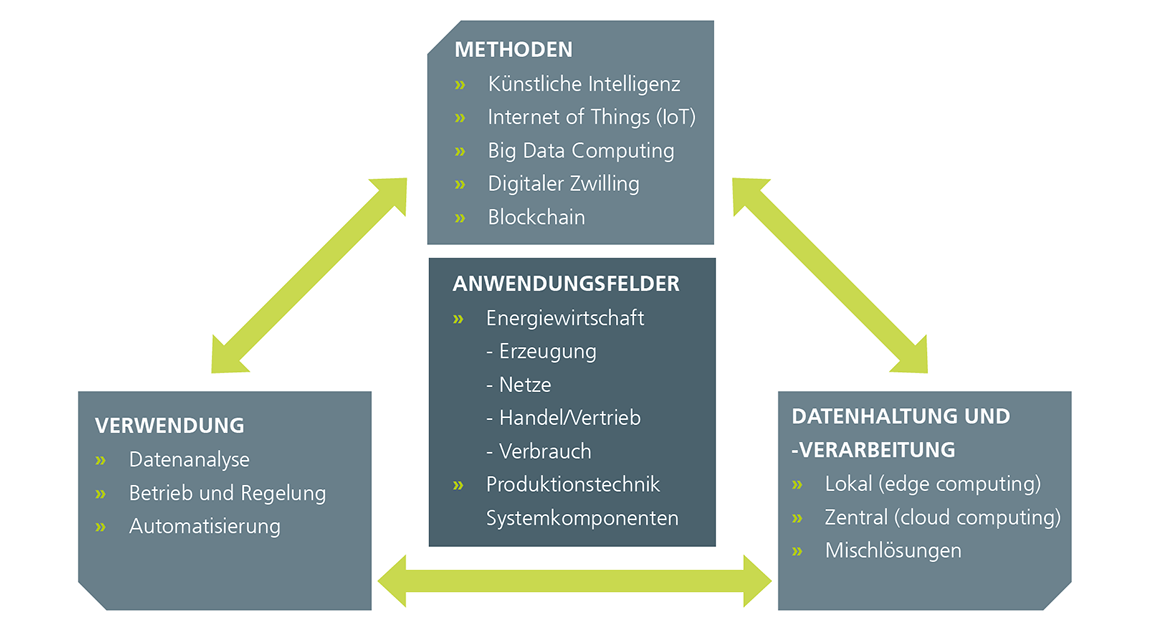
\includegraphics[width=1.0\linewidth]{dimensionen_digitalisierung_fraunhofer.png}
  \caption[Dimensionen der Digitalisierung]{Dimensionen der Digitalisierung \citep{FraunhoferISE}}
\end{figure}

\subsubsection{Allgemeine Anforderungen zur Umsetzung von Industrie 4.0}\label{general}

Im Rahmen der Industrie 4.0, die eine Spezialisierung des Internet der Dinge und Dienste darstellt, wachsen die virtuelle und reale Welt zusammen. Daraus ergibt sich die Herausforderung, die Anforderungen der IT, der Elektrotechnik sowie des Maschinenbaus miteinander zu vereinen \citep{Huebner2017}.

Aufgrund der heterogenen Landschaften und Aussgangssituationen der Unternehmen sei eine Standardisierung der Technologien laut \citet{Bauer2014} unerlässlich. Des weiteren ist die Weiterentwicklung von Breitbandnetzwerken für eine echtzeitfähige Kommunikation von Systemen eine Grundvoraussetzung. Notwendig sind außerdem qualitätsgesicherte Dienste im Internet, die robust gegen Störungen sind. Der Begriff \textit{Internet der Dinge und Dienste} bezieht auf vernetzte Komponenten wie physische Systeme, aber auch auf virtuelle Anwendungen. Da sich die Anzahl und die Beschaffenheit der Applikationen ebenso rasant ändern kann wie die der Geräte, sind eine standardisierte Laufzeitumgebung und Kommunikation für diese von großer Bedeutung. Nicht zu vernachlässigen sind dabei die Sicherheitsaspekte. Die \ac{iot}-Anwendungen bilden eine große Angriffsfläche für Hacker, die durch Sabotage und Manipulation der Systeme eine große Gefahr dartellen. Ein historisches Beispiel für solch eine Gefahr sind die Stuxnet-Angriffe von 2010 auf iranische Atomfabriken \citep{Bauer2014}.

Allgmein können die Anforderungen und Voraussetzungen für eine \ac{iot}-Lösung auf folgende Begriffe projiziert werden \citep{Acharya2019}:

\begin{itemize}
  \item Skalierbarkeit und Flexibilität
  \item Schnelligkeit
  \item (Ausfall-)Sicherheit
  \item Qualität
\end{itemize}

\subsubsection{Standardisierung und Normung}\label{rami}

Für die Bewältigung der oben aufgeführten Herausforderungen veröffentlichte die Plattform Industrie 4.0 das \glqq Referenzarchitekturmodell Industrie 4.0\grqq{} (RAMI 4.0) sowie das Konzept zur \glqq Industrie-4.0-Komponente\grqq{}. Beide Modelle wurden 2016 nach DIN SPEC 91345 der Standardisierung zugeführt \citep{Beuth2016}.

\paragraph{RAMI 4.0} ist ein branchenübergreifendes Rahmenwerk, in dem Aufgaben und Abläufe der gesamten Wertschöpfung in überschaubare Teile zerlegt und entsprechenden Normen und Standards zugeordnet werden. Das dreidimensionale Modell ist in Anlehnung auf das Smart Grid Modell erstellt und kapselt die wichtigsten Funktionalitäten aus den verschiedenen Disziplinen in Schichten. Dies schafft Flexibilität für die Konzeptionisierung und Realisierung von Industrie-4.0-Lösungen \citep{Huebner2017}.
\\
Für die Migration von Produktionsgegenständen von der heutigen in die Industrie"=4.0"=Welt soll der gesamte Prduktlebenszyklus in Daten erfasst und IT"=seitig einheitlich und durchgängig abgebildet werden. Die senkrechte Achse behandelt die IT"=Sicht, die die vertikale Integration der Assets in die Geschäftslogik und deren echtzeitfähige Vernetzung im Produktionsprozess beschreibt. Zu den Assets werden sowohl alle in der Anlage verbauten physischen Komponenten als auch andere Vermögensgegenstände wie Software oder Patente, aber auch Menschen, gezählt \citep{Adolphs2017}. Mit der Ergänzung des Assets um eine \textit{Verwaltungsschale} entsteht die \textit{Industrie-4.0-Komponente}. Die Verwaltungsschale ist das Bindeglied zwischen der realen und der virtuellen Welt. Mit dessen Hilfe wird ein virtuelles Abbild des Assets samt der dazugehörigen Funktionen und Daten erzeugt. Die IT-technische Beschreibung ermöglicht die eindeutige Identifizierung des Assets z.B. durch die \ac{uri}-Adresse im gesamten Wertschöpfungsprozess. Die Aktivitäten für den Übergang in die virtuelle Welt sind in der Integrantionsschicht enthalten. Die Dienste zur Steuerung der Integration werden von der Kommunikationsschicht bereitgestellt. Sie dient außerdem der Vereinheitlichung der Kommunikation mit einem einheitlichen Datenformat \citep{BITKOM2015}. Für die Datenkommunikation wird der Standard für industrielle Kommunikation \ac{opcua} empfohlen. Ursache dafür ist zum einen die plattformunabhängige, \ac{soa} und zum anderen die Fähigkeit, die Maschine"=zu"=Maschine"=Kommunikation semantisch zu beschreiben.
Anschließend werden die übertragenen Daten in der Informationsschicht gehalten, wo sie in einer Laufzeitumgebung in einen Regelkontext gebracht werden. Hier werden Regeln für Ereignisse und den Zugriff auf Daten definiert, die in der Funktionsschicht verarbeitet werden. Die tatsächlichen Funktionen eines Assets werden in der Funktionsschicht formal beschrieben. In der funktionalen Schicht befinden sich die Daten in einer Laufzeit- und Modellierungsumgebung für Dienste, die unter anderem Geschäftsprozesse unterstützen. Mit dieser Plattform können die Funktionen horizontal in die Wertschöpfung integriert werden \citep{Huebner2017}. Zusätzlich kann in der Funktionssicht auf ERP-Funktionen zugegriffen werden. Diese entstehen in der Geschäftssicht, in der die Modellierung der Regeln für die Geschäftsprozessabwicklung stattfindet. Letztendlich werden die Assets und deren Funktionen hier in die Organisation und Geschäftsprozesse integriert.
\\\\
Jede dieser IT-Schichten liegt an zwei wagerechten Achsen an, welche die horizontale Integration der Produktionsgegenstände in den gesamten Produktionprozess beschreiben. Die linke Achse soll den gesamten Lebenszyklus von Assets abbilden, während die rechte Achse diese in Hierarchiestufen der Produktions- und Automatisierungstechnik anordnet. Somit können externe Akteure wie Lieferanten oder Kunden, aber auch das erzeugte Produkt in das Industrie-4.0-Netzwerk aufgenommen werden \citep{BITKOM2015}.


% ************* CLOUD COMPUTING ******************
\subsubsection{Das neue Paradigma: Cloud Computing}

Flexibilität, Skalierbarkeit, Schnelligkeit, Sicherheit und Qualität präsentieren sich als die wichtigsten Voraussetzungen für die erfolgreiche digitale Transformation eines Unternehmens \citep{Acharya2019}. Für die Erzielung dieser Ziele spielt die in \ref{technologien} bereits kurz erläuterte Cloud eine Schlüsselrolle. Denn die Technologien in der Industrie 4.0 sind zwar nicht neu, aber sie müssen in verschiedenen Kombinationen bei niedrigen Preisen und unabhängig vom Ort stets verfügbar sein. Bei alledem wird dem Nutzer je nach Bedarf das Errichten von IT-Infrastruktur und IT-Ressourcen von dem Cloud-Dienstleister abgenommen \citep{Dzombeta2017}. Entsprechend können die Cloud-Dienste aus folgenden Varianten nach nutzungsbasierten Abrechnungsmodellen wie z.B. dem Pay-Per-Use-Prinzip erworben werden:

\paragraph{\ac{iaas}} Bei dieser Variante stellt das Dienstleistungsunternehmen die notwendige Hardware in virtueller Form zur Verfügung. Es können je nach benötigter Menge Speicherplatz, Prozessorleistung oder Netzkapazitäten bestellt oder wieder abbestellt werden \citep{Dzombeta2017}. Kostentechnisch bietet das einen großen Vorteil, da die Server von den Anbietern angeschafft, betrieben und gewartet werden, sodass nur die verbrauchte oder vereinbarte Kapazität in Rechnung gestellt wird. Zu den global dominierenden Anbietern gehören Amazon, Microsoft und Google, die in Nordamerika, Europa und Ostasien eine hohe Dichte an Rechenzentren aufweisen \citep{Acharya2019}.

\paragraph{\ac{paas}} Das Dienstleistungsangebot dieser Variante beläuft sich auf die Bereitstellung von Middleware, Laufzeit- und Entwicklungsumgebungen zur Erstellung von Anwendungen, Datenbanken und Webservices. Über definierte Schnittstellen (APIs) kann auf die Entwicklungsumgebung zugegriffen werden \citep{Dzombeta2017}. Da die Plattform auf \ac{iaas} basiert, fällt die Administration von Servern weg \citep{Acharya2019}.

\paragraph{\ac{saas}} Kunden können bei dieser Form meist über Webbrowser auf Software(-pakete) zugreifen, die auf der Infrastuktur des Anbieters gehostet sind. Dabei übernimmt der Anbieter Aufgaben wie Installation, Wartung und Aktualisierung der Software \citep{Utecht2018}. Dieses Prinzip ermöglicht einen schnellen Einsatz sowie eine einfache Austauschbarkeit der Software bei niedrigen Kosten. Aufgrund der Unabhängigkeit von lokalen Installationen kann die Software ortsunabhängig bei verfügbarer Internetverbindung genutzt werden \citep{Dzombeta2017}.

\vspace{0.5cm}
\noindent Die verschiedenen Modelle könnten auch in Kombination mit dem On-Premise-System genutzt werden.

\newpage

\noindent Mit diesen Modellen bietet die Cloud einen Raum für die verschiedenen Teilsysteme, die im Industrie"=4.0"=Netzwerk miteinander kommunizieren und Dienste anbieten. Eine \acf{soa} ermöglicht die Interoperabilität der Akteure wie Komponentenhersteller, Automatisierer, Maschinenbauer und Softwarefirmen ohne Master"=Slave"=Beziehungen. In der \ac{soa}-Welt wird nicht mehr zwischen Hard- und Software unterschieden, sodass maschinelle Komponenten ihre Daten genau so als Service zur Verfügung stellen können wie eine Software ihre Funktionen bereitstellt \citep{Adolphs2017}. Entwicklungen wie diese verändern die grundsätzliche Denkweise in der Softwareentwicklung. Alte Architekturen werden von neuen Architekturen wie die \textit{Microservice-Architektur} vertrieben \citep{Acharya2019}.

\begin{figure}[]
  \centering
  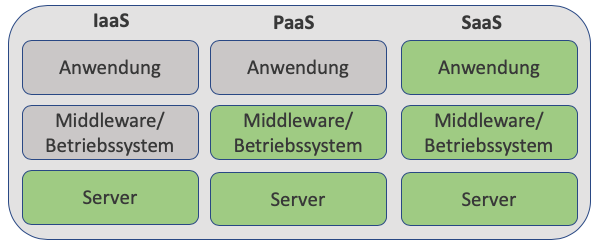
\includegraphics[width=0.8\linewidth]{cloud_variant.png}
  \caption[Die Cloud-Service-Modelle]{Die Cloud-Service-Modelle (In Anlehnung an \citet[S. 88]{Utecht2018})}
  \label{}
\end{figure}

\paragraph{Cloud-native-Anwendungen und Microservices}

Die Eigenschaft cloud-nativ besitzen jene Anwendungen, welche in der Cloud \glqq geboren\grqq{} sind und durch Auschöpfung des Cloud"=Potenzials die Flexibilität, Agilität und Skalierbarkeit von Cloud-Lösungen unterstützen \citep{Acharya2019}. Besonders ist dabei der agile und schnelle Entwicklungsprozess der Software. Eine cloud"=native Anwendung besteht aus mehreren isolierten Services, die unabhängig voneinander entwickelt werden können. Konventionelle Anwendungen sind im Gegensatz dazu monolithischer Natur und basieren meist auf der 3"=Tier"=Architektur. Mit den Bestandteilen Benutzeroberfläche, Datenbank und Anwendungsserver bilden sie ein geschlossenes System. Kleinste Änderungen an einem der Bestandteile führen zu aufwendigen Maßnahmen zur Anpassung des Gesamtsystems \citep{Utecht2018}.
Anders als monolithische Architekturen zeichnet sich die Microservice-Architektur durch ihre einfache und schnelle Erweiterbarkeit und Anpassungsfähigkeit aus. Ein Microservice ist eine spezielle Funktion, oft Geschäftsfunktion, welche in Containern in in einer isolierten Umgebung ausgeliefert wird und meist an eine eigene Datenbank angebunden ist. In einer Anwendung kommunizieren diese Microservices über APIs oder Messaging"=Prokolle miteinander und bilden ein Gesamtsystem mit heterogenen Datenquellen. Sollte eine Funktion ein Update erforden, muss lediglich der Microservice  gewartet werden. Wenn das System eine neue Funktion erfordert, kann ein neuer Microservice einfach hinzugefügt werden, ohne Abhängigkeiten im Gesamtsystem zu stören. Infrastrukturressourcen können bei Bedarf dynamisch zu- oder abgewiesen werden \citep{Acharya2019}.



\subsubsection{Der Wandel im Energiesektor}
Welche Veränderungen durchlebt der Energiesektor?
Mechanisierung, Automatisierung und Digitalisierung sind die Schlagworte des industriellen Wandels, der auch die Energiewirtschaft betrifft.


Hier könnte man Bezug auf Energiesektor (kurz) nehmen und einführen, mit welchen Anforderungen und technologien generell so ein Wandel/Transformation stattfinden kann.
\begin{itemize}
  \item Disruption bestehender Geschäftsmodelle, vom Produzenten zum Dienstleister \citep{Doleski2017}
  \item dezentrale und fluktuierende Energieerzeugung erfordert digitale Lösungen
  \item wichtige Rolle kommunaler Unternehmen als Bereitsteller von Infrastrukturen wie Strom, Gas, Wärme, Wasser, Abwasser, Abfallwirtschaft, Stadtreinigung, Breitband \citep{Doleski2017}
  \item Beitrag zu funktionierendem Gemeinwesen, sozialer Teilhabe und Versorgungssicherheit -> Partner erster Wahl beim Gelingen der digitalen Transformation
  \item Wichtig für Gelingen: Erfahrungsaustausch, Kooperationen, richtige politische Rahmenbedingungen -> Katherine Reiche
  \item auf Unternehmensseite: Aufbau und Umsetzung einer unternehmensspezifischen Digitalisierungsstrategie: RAMI 4.0 als Referenz möglich
  \item Drei Revolutionen in der Energiewirtschaft \citep{Doleski2017}
  \begin{enumerate}
    \item Ab 1998: Liberalisierung und Privatisierung der Strommärkte fördert Wettbewerb, stellt aber eine Herausforderung Digitalisierungsstrategie
    \item Ab 2011: Energiewende und Aussteig aus Kernenergie fördert neue Technologien für erneuerbare Energien, aber die Berechenbarkeit der Kapazitäten verändert sich
    \item Digitalisierung: Potenzial für neue Revolution, Strom kann zwar nicht digitalisiert werden, aber die Vertriebsmodelle
  \end{enumerate}
  \item Datenschutz und Sicherheit gewinnen an Bedeutung
  \item Trend: Energieversorgungsunternehmen wandeln sich Richtung Dienstleitsungsunternehmen
  \item \glqq Mit der Zunahme dezentraler Einspeisungs- und Eigenversorgungsanlagen innerhalb der bestehenden Strom- und Gasnetze steigen synchron auch die Koordinationsanforderungen und die zu beherrschenden Datenmengen \grqq{} \citep[S. 7]{Doleski2016}
  \item \glqq Bedarf einer branchenweiten Veränderung - einer Transformation - in allen Sektoren und Phasen entlang der energiewirtschaftlichen Wertschöpfung\grqq{} \cite[S. 11]{Doleski2016}
  \item Utility 4.0: Digitale Enegergiedienstleistungsunternehmen
  \item Während nach Dampfmaschine, Massenproduktion und Automation nunmehr die Digitalisierung die vierte industrielle Revolution einläutet, unterliegt die Energiewirtschaft ähnlichen Entwicklungsprozessen.
\end{itemize}

\begin{figure}[h]
  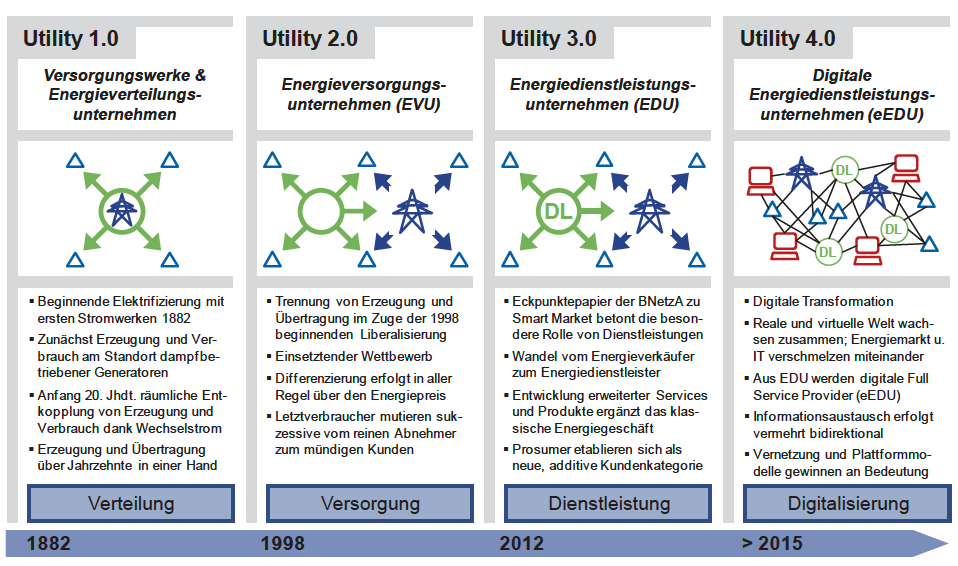
\includegraphics[width=1.0\linewidth]{utility_40.png}
  \caption[Transformation vom Versorgungswerk zum digitalen Energiedienstleister]{Transformation vom Versorgungswerk zum digitalen Energiedienstleister \citep[S. 13]{Doleski2016}}
\end{figure}

\begin{figure}[h]
  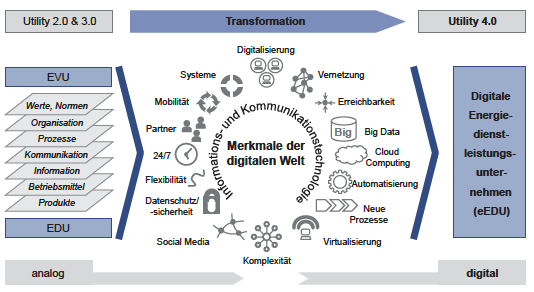
\includegraphics[width=1.0\linewidth]{kalalysator_utility_40.png}
  \caption[Digitale Welt als Katalysator für Utility 4.0 ]{Digitale Welt als Katalysator für Utility 4.0 \citep[S. 17]{Doleski2016}}
\end{figure}
